\subsection{SyntaxSQLNet 2018}
% [2] Yu, Tao, et al. “Syntaxsqlnet: Syntax tree networks for the complex and cross-domain text-to-SQL task.” arXiv preprint arXiv:1810.05237 (2018).

The main\cite{DBLP:journals/corr/abs-1810-05237} goal of developing the SyntaxSQLNet model was to generate complex SQL queries with multiple clauses and generalize them to new databases.
This was achieved through the use of a syntax tree network, which is capable of addressing complex and cross-domain queries.

As is evident in the chart below, the SyntaxSQLNet model is composed of several components, each with its unique function and purpose in generating complex SQL queries. The encoders are table-aware, while the decoders have a history of the SQL generation path.

With a massive 7.3\% improvement in accuracy, SyntaxSQLNet outperformed previous models, such as SQLNet, on the SPIDER dataset.

A cross-domain data augmentation technique was employed to improve accuracy further to generate more variance during training, allowing for a greater degree of accuracy and robustness.

\begin{figure}[htb]
    \centering
    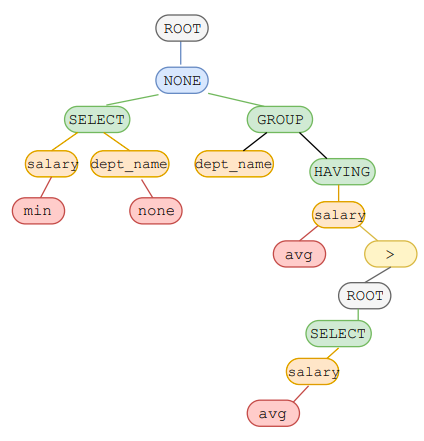
\includegraphics[width=0.6\textwidth]{pics/SyntaxSQLNet/Tree-based.png}
    \caption{Tree-based SQL generator in SyntaxSQLNet}
    \label{fig:tree-based}
\end{figure}

\begin{figure}[htb]
    \centering
    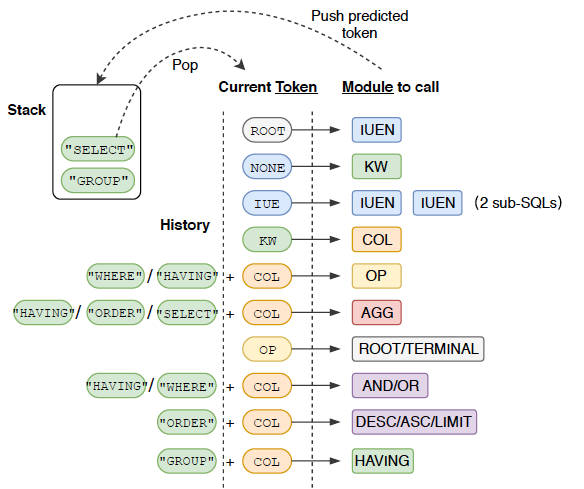
\includegraphics[width=0.8\textwidth]{pics/SyntaxSQLNet/Grammar.png}
    \caption{Modules defined in SyntaxSQLNet model}
    \label{fig:grammar}
\end{figure}


\textbf{SQL Grammar and Attention Mechanism}

In order to enable the decoder to handle complex queries, SQL grammar is used. This allows the decoder to make decisions at each step of recursive decoding, determining which module to invoke.

Furthermore, the prediction of the following SQL token is based on the history of SQL path generation and the current SQL tokens.

Additionally, the attention mechanism encodes the question representation and applies it to the SQL path history encoding.

This is beneficial as the history of SQL path generation can be used to determine which token should be used next. Thus, the attention mechanism helps to create a better representation of the query, allowing for an efficient and accurate response.

% \begin{figure}[htb]
%     \centering
%     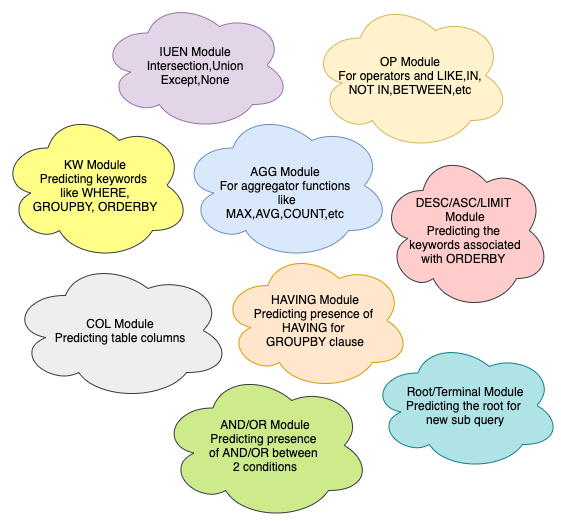
\includegraphics[width=0.8\textwidth]{pics/SyntaxSQLNet/Modules.png}
%     \caption{Modules and SQL Grammar used in the decoding process}
%     \label{fig:modules}
% \end{figure}


\textbf{Data Augmentation}

\begin{itemize}
    \item Despite SPIDER's large dataset, it lacks complex queries.
    \item For proper generalization, cross-domain datasets are used for data augmentation.
    \item Various training databases of the SPIDER dataset are used to prepare a list of patterns for natural language questions and corresponding SQL queries.
\end{itemize}

The SPIDER model using syntaxSQLNet decoding history reaches 27.2\% accuracy.


Compared to previous models, such as SQLNet, the accuracy increased by 15\%.